% \section{Results \& Discussions}

\section{Results and Discussions}
\label{sec:results}

We organize our results around three questions: \emph{which agents improve CWVs without causing regressions?} (\S\ref{sec:pareto-results}), \emph{does the agent framework or the LLM matter more?} (\S\ref{sec:ablations}), and \emph{what qualitative differences in planning and patching explain the performance gap?} (\S\ref{sec:qualitative}).

\subsection{Pareto CWV Improvement}
\label{sec:pareto-results}

We report the four metrics defined in \S\ref{sec:eval-metrics}: Pareto Rate, Net Threshold Crossing, Health Delta, and Degraded Sites which jointly capture improvement, tier transitions, and regression risk.

\begin{table}[t]
\centering
\small
\caption{Agent performance on 300 websites. \textbf{Pareto Rate}: fraction of sites where $\geq$1 metric improves meaningfully with no metric degrading beyond noise. \textbf{Net Threshold}: mean count of CWV category transitions across sites (Poor$\to$Good\,=\,+2, Good$\to$Poor\,=\,$-$2). \textbf{Health $\Delta$}: change in composite Site Health Score (\S\ref{sec:site-health}). Agents sorted by composite rank.}
\label{tab:main-results}
\begin{adjustbox}{max width=0.48\textwidth}
\begin{tabular}{lccccc}
\toprule
\textbf{Agent} & \textbf{LLM} & \textbf{Pareto} & \textbf{Net} & \textbf{Health} & \textbf{Degraded}  \\
 &  & \textbf{Rate (\%)}$\uparrow$ & \textbf{Thresh.}$\uparrow$ & \textbf{$\Delta$}$\uparrow$ & \textbf{Sites (\%)}$\downarrow$  \\
\midrule
OpenCode  & GPT-5.1\,Cdx & \textbf{56.7} & \textbf{+0.93} & \textbf{+7.4} & \textbf{20.0} \\
OpenCode  & GPT-5        & 53.3          & +0.93          & +7.4          & 23.3 \\
Codex     & GPT-5        & 36.7          & +0.60          & +3.0          & 20.0 \\
Claude~Code & Son.\,4.5   &  3.3          & $-$1.13        & $-$11.4       & 53.3 \\
Aider     & GPT-5        &  3.3          & $-$1.17        & $-$7.1        & 66.7 \\
OpenCode  & GPT-4.1      &  0.0          & $-$2.17        & $-$16.5       & 90.0 \\
\bottomrule
\end{tabular}
\end{adjustbox}
\end{table}

\subsection{Measuring Agency}


\subsection{Agent vs.\ LLM Ablations}
\label{sec:ablations}

Our experimental design enables two clean ablations that disentangle the contributions of the agent scaffold from the underlying language model. Figure~\ref{fig:radar-ablation} visualizes both ablations as radar plots over the six-dimensional Site Health Score space.

\begin{figure}[t]
    \centering
    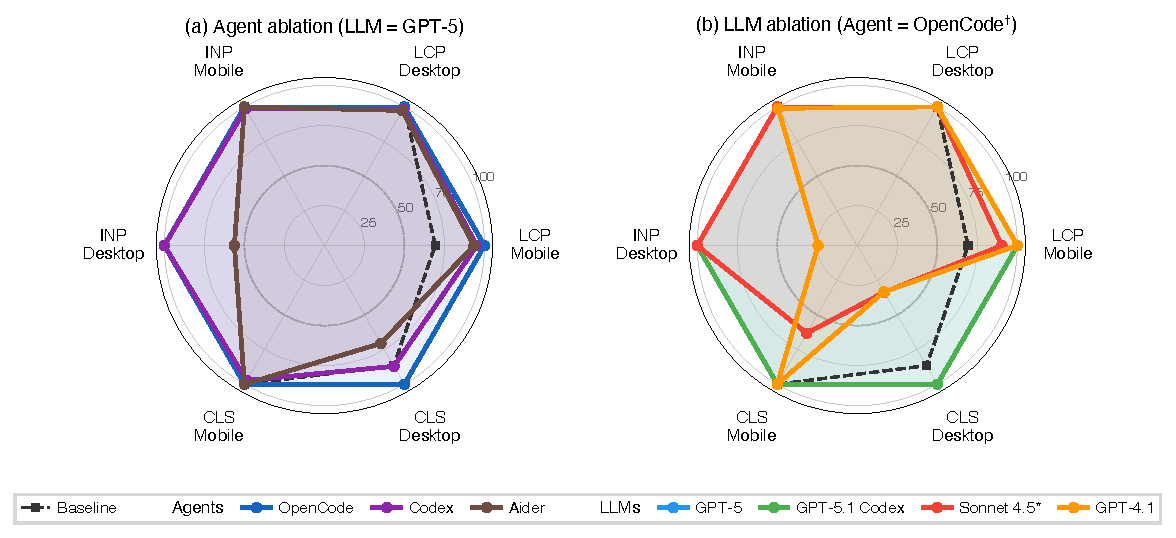
\includegraphics[width=\linewidth]{figures/fig_radar_ablation.pdf}
    \caption{Site Health Score radar for the two ablation conditions, averaged across 300 websites (higher = healthier; 100 = at or below the CWV Good threshold, 50 = Needs Improvement boundary). \textbf{(a)}~Agent ablation with GPT-5 fixed: OpenCode's polygon fully envelops the baseline on all six axes, while Aider collapses on INP~Desktop, revealing the importance of the planning phase. \textbf{(b)}~LLM ablation with the agent scaffold held to plan-then-implement systems (OpenCode for GPT-5/5.1\,Codex/4.1; Claude~Code$^{\dagger}$ for Sonnet\,4.5 as an architecturally comparable proxy): GPT-5 and GPT-5.1\,Codex envelop the baseline whereas GPT-4.1 collapses on INP/CLS~Desktop and Sonnet\,4.5 collapses on CLS~Mobile/Desktop, showing that model capability governs side-effect avoidance.}
    \Description{A two-panel radar chart comparing Site Health Score dimensions across ablations. The left panel compares agent frameworks with GPT-5 fixed, where OpenCode dominates the other agents. The right panel compares language models under a matched scaffold, where GPT-5 and GPT-5.1 Codex outperform GPT-4.1 and Sonnet 4.5 on preserving overall metric health.}
    \label{fig:radar-ablation}
\end{figure}

\paragraph{Agent ablation}
Holding the LLM fixed at GPT-5, we compare OpenCode, Codex, and Aider (Figure~\ref{fig:radar-ablation}a).
OpenCode achieves 53\% Pareto rate, Codex 37\%, and Aider 3\%, a 16$\times$ gap between the best and worst agent frameworks using the identical model, while Aider causes INP-Desktop regressions on 66\% of sites.

\paragraph{LLM ablation}
To isolate the effect of the LLM, we compare three LLMs under OpenCode and additionally include Claude-Code with Sonnet\,4.5 as an architecturally comparable proxy.  GPT-5 and GPT-5.1 Codex, improve LCP while preserving all other metrics. GPT-4.1's collapses dramatically on INP-Desktop and CLS-Desktop despite matching GPT-5 on LCP (median normalized gain of +0.56 vs.\ +0.59; Appendix~\ref{app:per-metric}).

Taken together, the two panels indicate that \emph{both} the agent scaffold and the LLM contribute to Pareto performance, but in complementary ways: the scaffold determines whether the system can plan and structure multi-metric trade-offs, while the model determines whether it has the judgment to execute that plan without regressions, we further discuss some qualitative examples.

\subsection{Qualitative Analysis v1}
\label{sec:qualitative}
\arnav{maybe remove the ending sentences of every para so we can fit in 8 pages}

To understand the mechanisms behind the quantitative gaps, we analyzed the plans, patches, and agent logs produced for 120 representative websites spanning sites with Poor LCP baselines requiring improvement, mixed-metric profiles, and sites where all metrics are already Good. We report quantitative patch statistics across all 300 sites and qualitative findings from targeted case studies.

\subsubsection{Precision Over Volume}
Table~\ref{tab:patch-stats} reports patch-level statistics. The most striking pattern is the \emph{negative} correlation between patch size and Pareto improvement rate. OpenCode+GPT-5 adds a median of 63 lines of code per webpage and achieves 53\% Pareto rate; OpenCode+GPT-4.1 adds a median of 48 lines but makes modifications inside files far more aggressively (1{,}242 mean lines with 1{,}133 removals, indicating wholesale file rewrites); Claude-Code adds a median of 55 lines but touches 34 files per site on average with 927 mean additions. The top agents make \emph{surgical} changes to 4-5 files while the bottom agents scatter modifications across up to 34 files.

\begin{table}[t]
\centering
\small
\caption{Patch and plan statistics (mean across 30 sites). Patch hunks counted as contiguous diff blocks; files modified counted from \texttt{diff --git} headers.}
\label{tab:patch-stats}
\begin{adjustbox}{max width=0.48\textwidth}
\begin{tabular}{lrrrrc}
\toprule
\textbf{Agent+LLM} & \textbf{Plan} & \textbf{Patch} & \textbf{Patch} & \textbf{Files} & \textbf{Pareto} \\
  & \textbf{Words} & \textbf{Lines+} & \textbf{Lines$-$} & \textbf{Mod.} & \textbf{(\%)} \\
\midrule
OC+GPT-5       & 999  & 100   & 82    & 4.6  & 53.3 \\
OC+GPT-5.1\,Cdx & 469  & 268   & 277   & 3.6  & 56.7 \\
Codex+GPT-5    & ---  & 92    & 101   & 6.1  & 36.7 \\
CC+Son.\,4.5    & 2264 & 927   & 388   & 33.9 &  3.3 \\
Aider+GPT-5    & ---  & 65    & 7     & 4.5  &  3.3 \\
OC+GPT-4.1     & 736  & 1242  & 1133  & 2.8  &  0.0 \\
\bottomrule
\end{tabular}
\end{adjustbox}
\end{table}

Plan verbosity also does not predict quality. Claude~Code produces the longest plans (2{,}264 words on average) but ranks fifth. OpenCode+GPT-5.1\,Codex achieves the highest Pareto rate with the most \emph{concise} plans (469 words)---roughly a fifth of Claude~Code's output. What distinguishes top-performing plans is not length but \emph{specificity}: GPT-5 plans reference exact file paths, script tag locations, and CSS selectors (e.g., ``\texttt{repo/index.html} lines 26--43: scripts loaded without \texttt{defer}''), whereas GPT-4.1 plans give generic prescriptions (``reduce render-blocking CSS,'' ``optimize images'') that could apply to any website.

A second distinguishing feature is \emph{risk awareness}. On site 2361 (LCP~Mobile = 8{,}548\,ms, all other metrics Good), GPT-5's plan explicitly notes: ``Desktop metrics are healthy (LCP $\sim$0.83s, INP p75 20ms), so changes should prioritize mobile and avoid regressions on desktop.'' GPT-4.1's plan for the same site makes no mention of preserving the already-Good metrics.

\subsubsection{Failure Modes}
\label{sec:failure-modes}

Patch analysis across the 12 case-study sites reveals three recurring failure modes that explain the majority of regressions.

\paragraph{Async CSS without layout protection (CLS regression).}
Claude~Code consistently converts render-blocking stylesheets to async loading using the \texttt{media="print" onload="this.media='all'"} pattern. While this unblocks rendering, it produces a Flash of Unstyled Content (FOUC) that generates CLS values of 0.86--1.08 on 16 of 30 sites. On site 813, for instance, baseline CLS~Desktop is 0.094 (Good); after Claude~Code's patch, it rises to 1.08 (Appendix~\ref{app:patch-813-cc}, Listing~\ref{lst:cc-813}). GPT-5 avoids this entirely---it keeps stylesheets render-blocking but adds a \texttt{<link rel="preload">} hint for the critical CSS file, achieving faster paint without FOUC.

\paragraph{Resource over-prioritization (INP regression).}
Agents that preload multiple assets with \texttt{fetchpriority="high"} cause main-thread contention. On site 404 (Appendix~\ref{app:patch-404-gpt41}, Listing~\ref{lst:gpt41-404}), GPT-4.1 preloads four thumbnail images simultaneously with high priority, competing with the actual LCP element for bandwidth and CPU time. This pushes INP~Desktop from 16\,ms to 752\,ms. GPT-5, by contrast, preloads only the identified LCP image and defers all others. Claude~Code exhibits an extreme variant: it adds 116 \texttt{preload} directives per site on average---47$\times$ more than GPT-5's 2.5.

\paragraph{Template application to already-Good sites.}
On sites where all metrics are already Good (e.g., site 952: LCP = 392\,ms, INP = 24\,ms, CLS = 0), the correct action is minimal or no intervention. Yet every agent applies optimizations. GPT-4.1's patch for site 952 references non-existent files (\texttt{styles.css}, \texttt{images/index-bg.webp}), generating 404 errors that block rendering (Appendix~\ref{app:patch-952-gpt41}). GPT-5 acknowledges the Good baseline in its plan (``Overall, scores are already in the Good range'') but still adds a sprite-caching system and \texttt{content-visibility} rules, causing a mild LCP regression of $\sim$200\,ms. No agent in our evaluation produces an empty patch for an already-optimal site, suggesting that all current systems lack a reliable ``do nothing'' judgment.

\subsubsection{Mechanism: Defer vs.\ Rewrite}

The single most effective LCP optimization in our dataset is adding the \texttt{defer} attribute to render-blocking \texttt{<script>} tags. GPT-5 performs this surgically---adding $\sim$9 defer attributes per site while leaving the rest of the page untouched. GPT-4.1 also defers scripts, but \emph{additionally} rewrites inline event handlers, restructures the DOM, and adds inline critical CSS, expanding the patch surface area and introducing regressions. On site 404, GPT-5 replaces jQuery \texttt{fadeIn}/\texttt{fadeOut} calls with CSS transitions (\texttt{opacity} + \texttt{transition: 150ms ease}), eliminating synchronous layout thrashing (Appendix~\ref{app:patch-404-gpt5}, Listing~\ref{lst:gpt5-404}). GPT-4.1 retains the jQuery animations, leaving layout-thrashing event handlers intact even after deferring the script.

This pattern---minimal, targeted modification vs.\ broad rewrite---is the clearest qualitative predictor of Pareto success. It suggests that the GPT-5-class models have learned a form of \emph{surgical restraint}: the ability to identify the minimal edit that improves the target metric without perturbing the rest of the system.